\documentclass{article} %选择文档类型,我们如果是做期末大作业的话选article就可以了
\usepackage{anyfontsize}
%正如c++需要import库来实现各种各样的功能,Latex也需要调用宏包来实现各种各样的功能
\usepackage{amsmath}  %调用公式宏包
\usepackage{graphicx} %调用插图宏包
\graphicspath{{code_Latex/}}
\usepackage{ctex}     %调用中文宏包
\usepackage{float}
\usepackage{cite}


%\begin{document}这句话之前是导言区,这句话以后就开始写正文了
%可以把导言区理解为int main()函数之前的内容,而正文就是int main()主函数的部分了
\usepackage{geometry}
\geometry{left=1.5cm,right=0.5cm,top=1.0cm,bottom=1.5cm}

\begin{document}
    \title{\centerline{数逻实验三报告}}
    \date{大二秋 实验三:数码管控制器}
    \author{信息学部计算机与电子通信7班 2023311704 王昕远 t2 612}
    \maketitle
    \thispagestyle{empty}


\section{数码管控制器}

信号说明:时钟信号clk,拨码开关按钮SW,复位按钮S1,计数器重置按钮S2,输入计数按钮S3,输出数码管编号led\_en,数码管显示数字led\_cx。\par

\section{仿真图像分析}
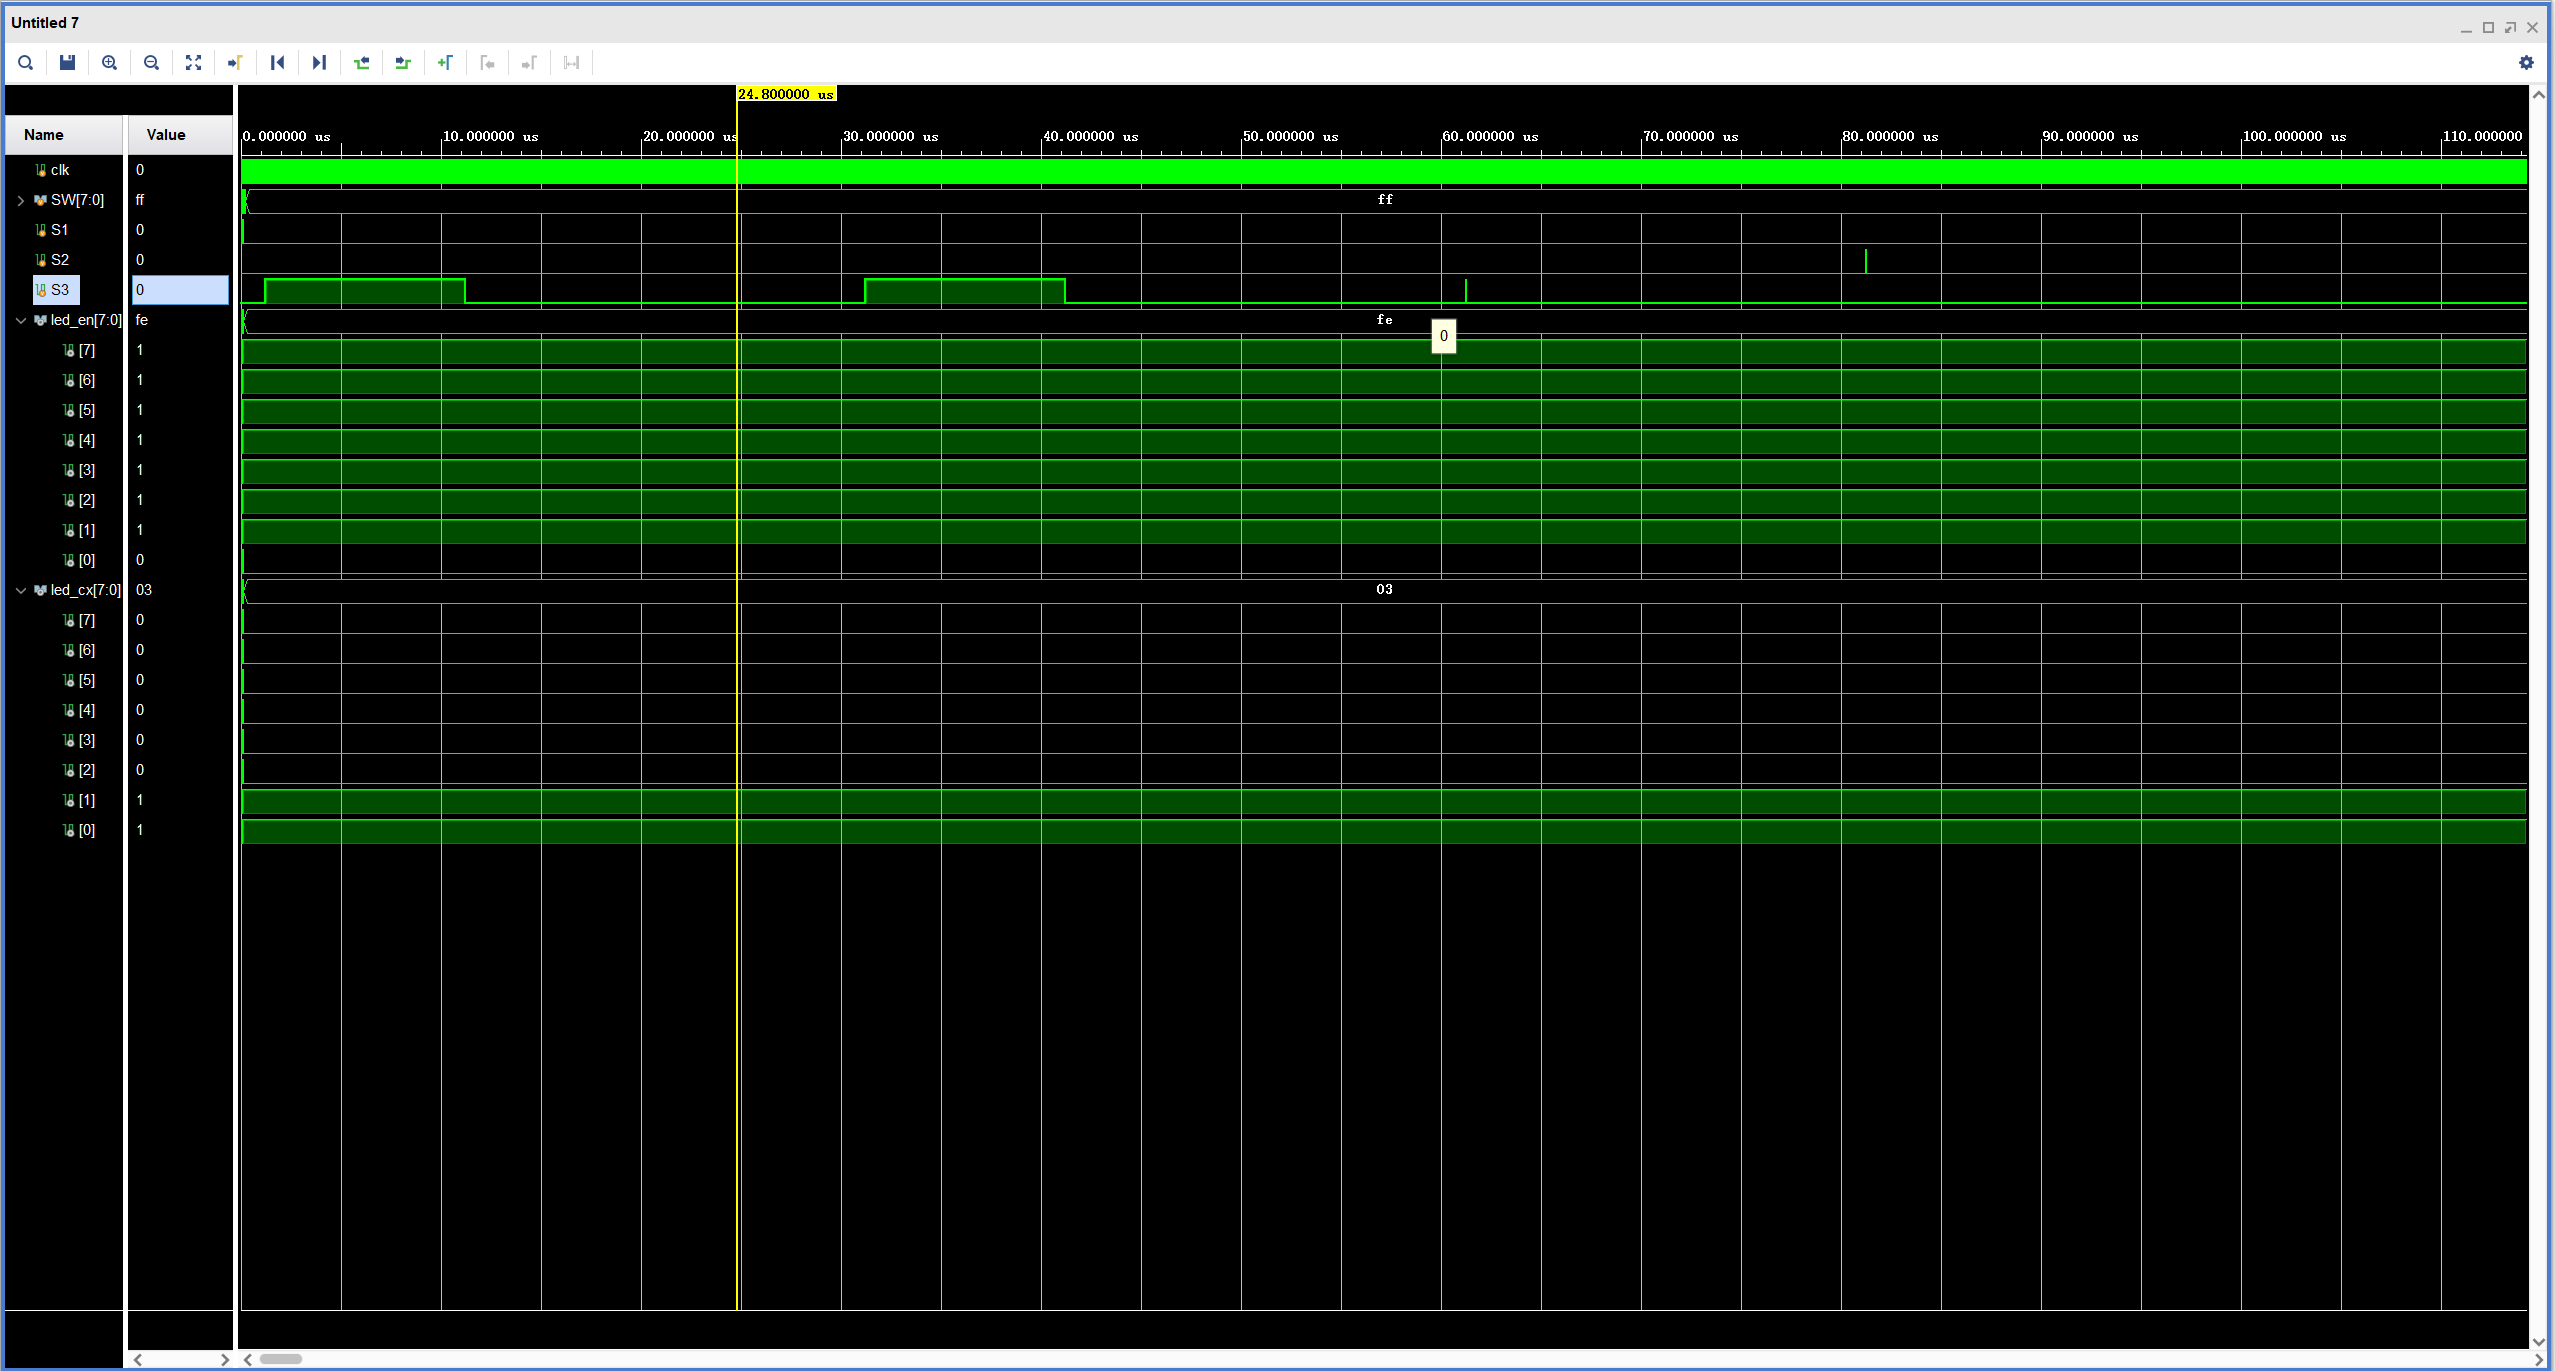
\includegraphics[width=0.8\textwidth]{sim2.png}\par
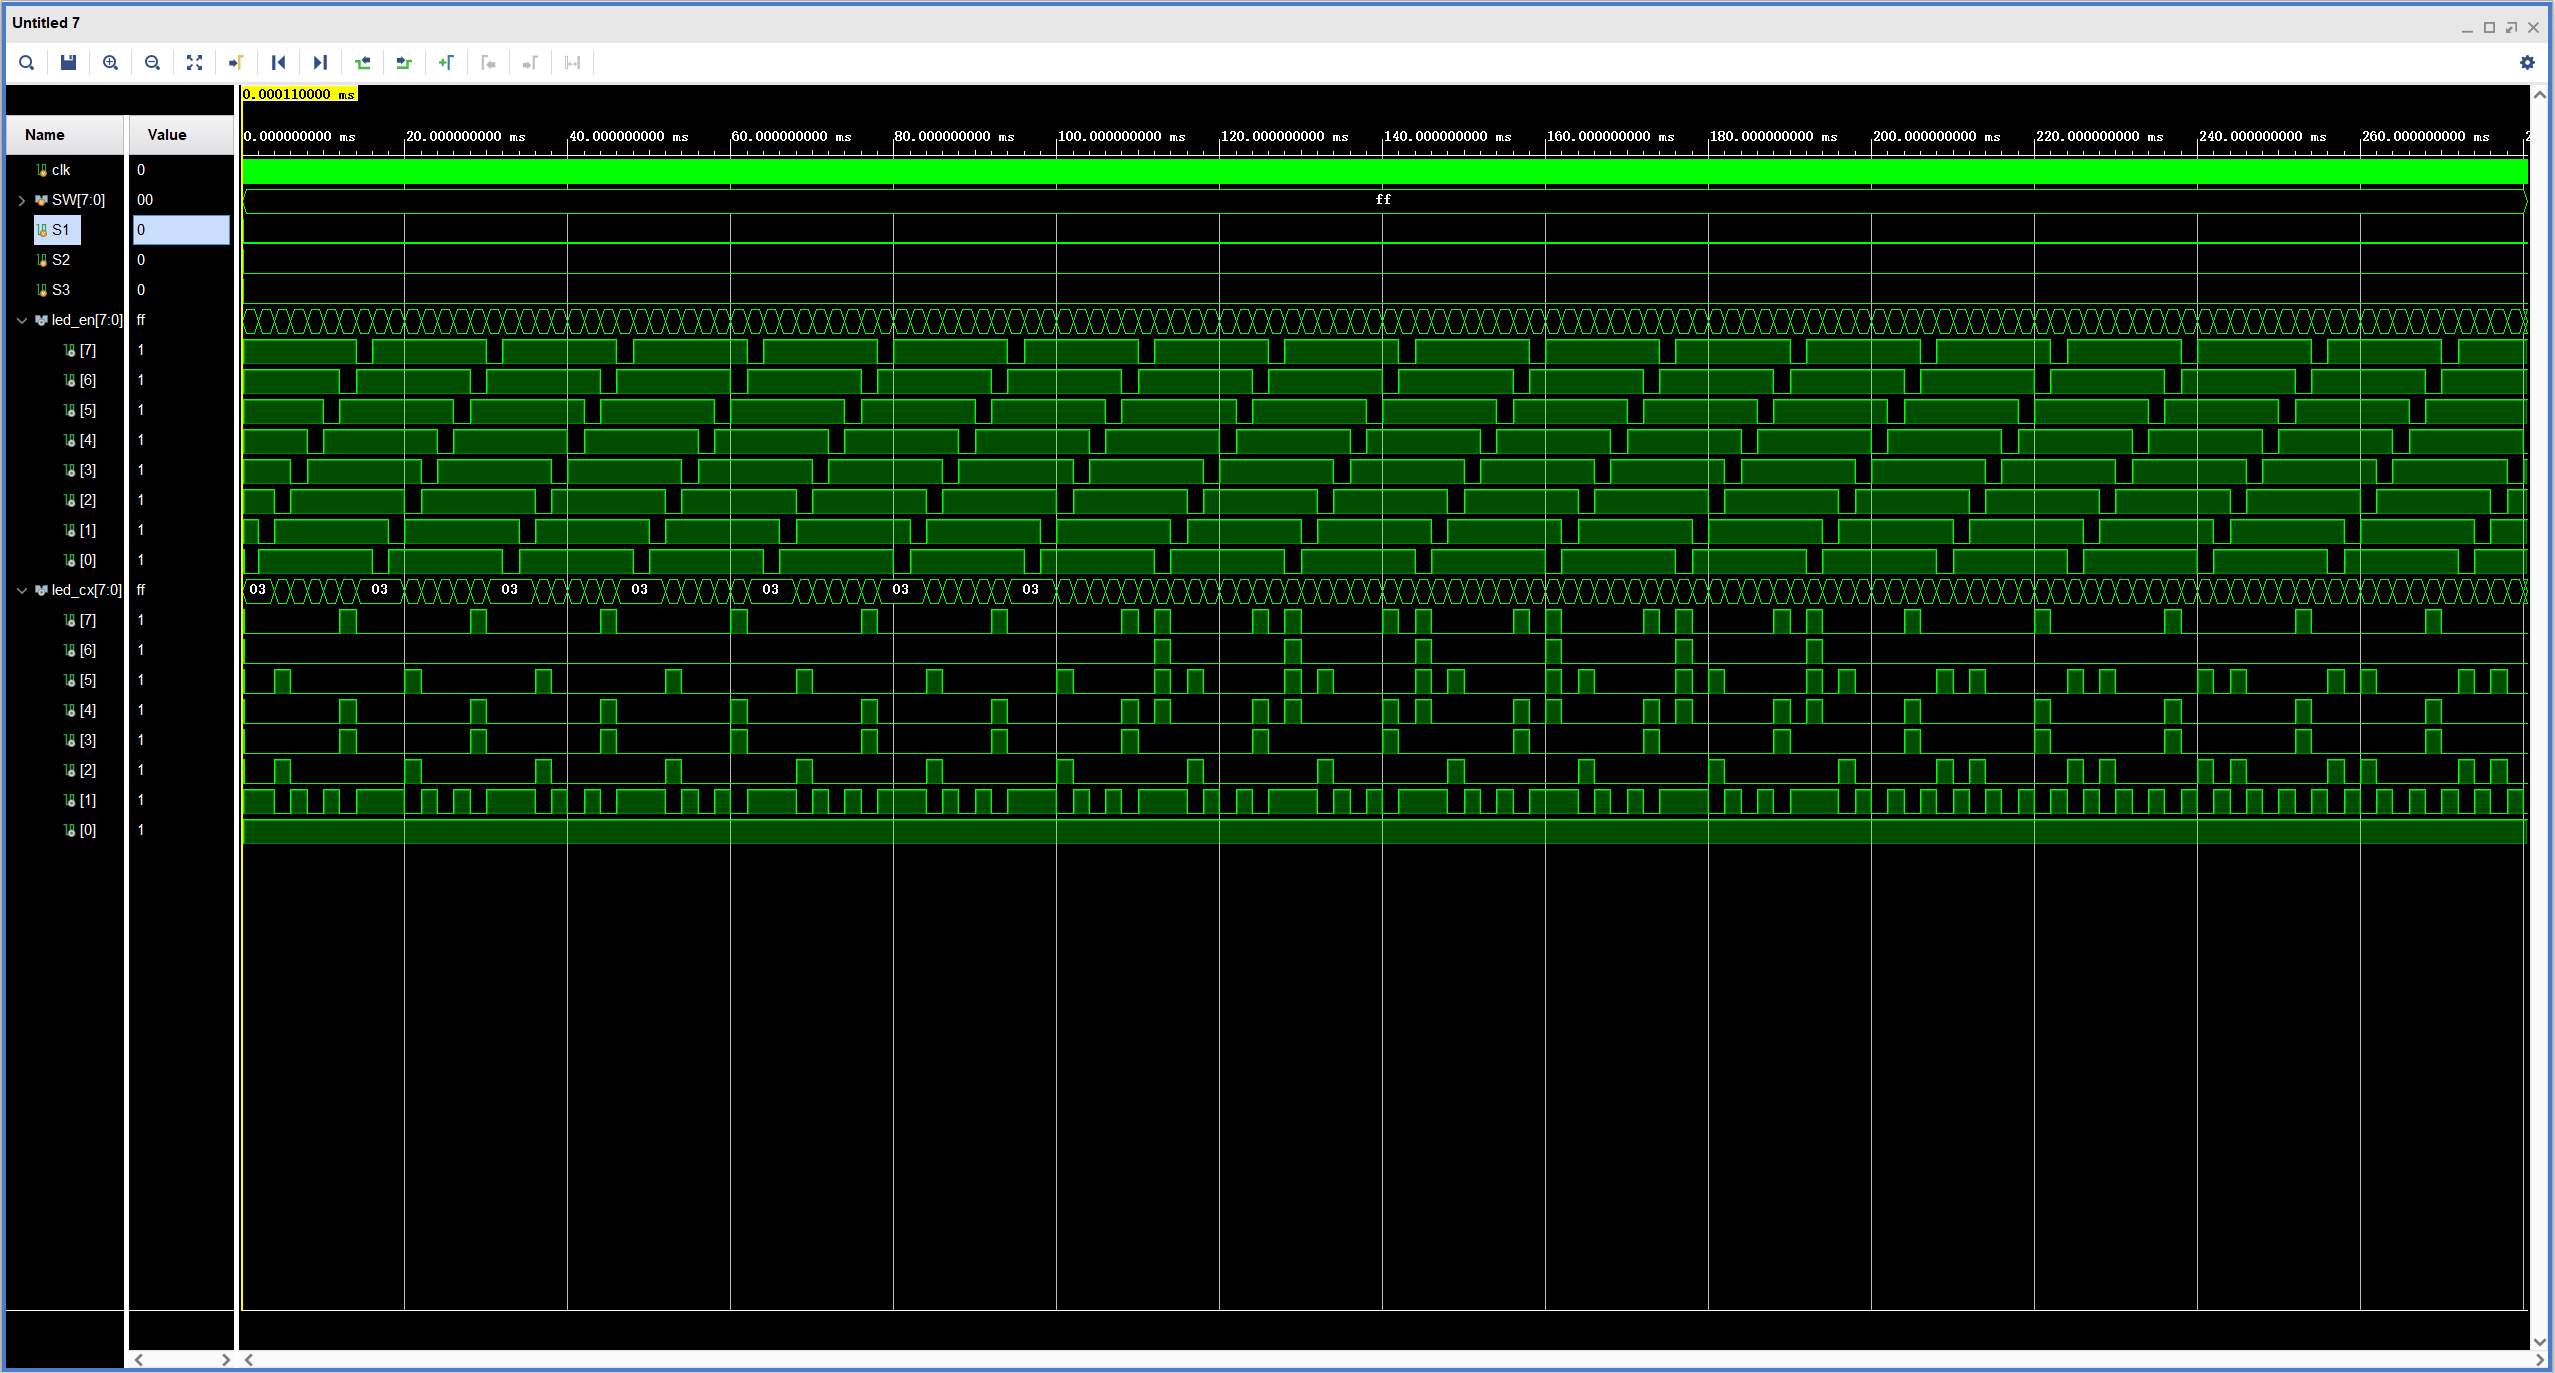
\includegraphics[width=0.8\textwidth]{sim1.png}\par
(1)摁两次正常的S3,摁一次极短(可以被视为毛刺剔除的S3)。\par
(2)led\_en7与led\_en6显示学号04\par
(3)将SW0-7全部置为1,输入1的个数为8,led\_en5与led\_en4显示08\par
(4)共有三次摁键S3输入,其中有效次数为两次,故led\_en3与led\_en2显示02\par
(5)led\_en1与led\_en0显示从0到20递增的计数器从00开始变化到20\par





\section{RTL Analysis}
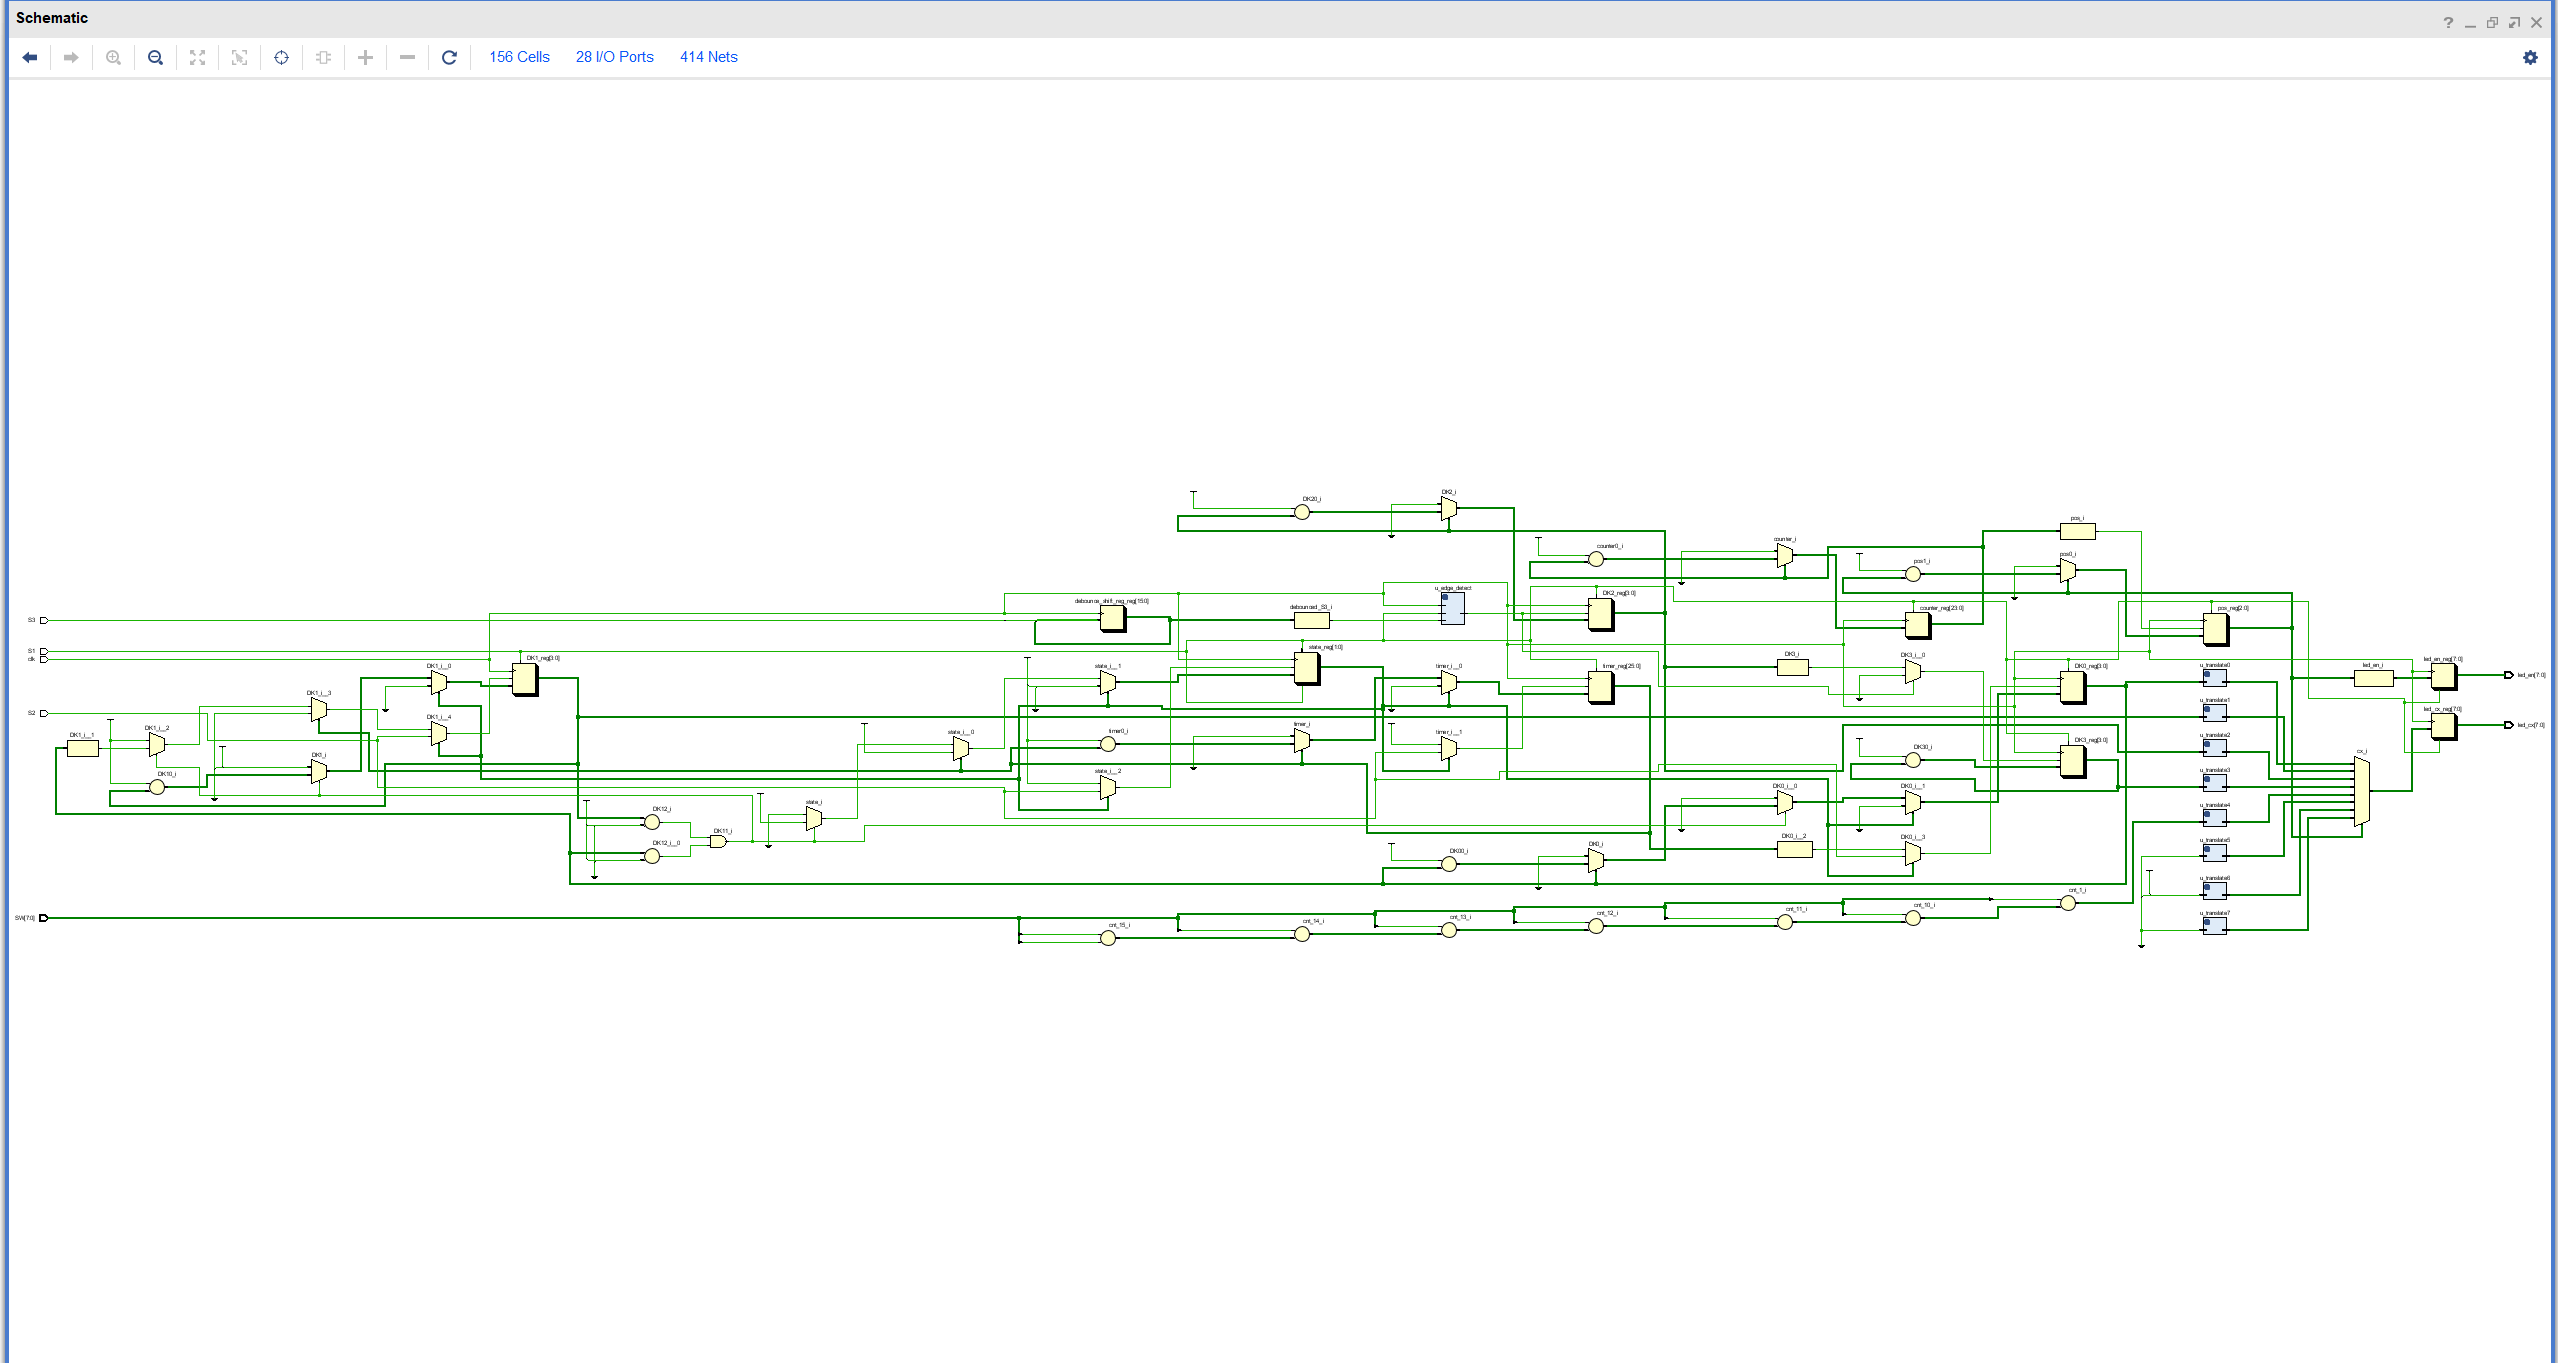
\includegraphics[width=0.8\textwidth]{RTL.png}\par
该图为RTL电路图,构成数码管控制器电路。\par


\section{数码管字符编码表}
\[
\begin{array}{|c|c|c|}
\hline
\text{Digit} & \text{编码} \\
\hline
0 & 8'b00000011 \\
1 & 8'b10011111 \\
2 & 8'b00100101 \\
3 & 8'b00001101 \\
4 & 8'b10011001 \\
5 & 8'b01001001 \\
6 & 8'b01000001 \\
7 & 8'b00011111 \\
8 & 8'b00000001 \\
9 & 8'b00001001 \\
a & 8'b00010001 \\
b & 8'b11000001 \\
c & 8'b11100101 \\
d & 8'b10000101 \\
e & 8'b01100001 \\
f & 8'b01110001 \\
\hline
\end{array}
\]
$$
$$



\end{document}